\documentclass{article}

\title{Notes on navigation history}
\author{%
  Alan Jeffrey
  \and
  Connor G.~Brewster
}
\date{DRAFT of 2016-06-16}

\usepackage{amssymb}
\usepackage{tikz}
\usetikzlibrary{fit}

% Macros, so we can change notation easily
\newcommand{\aNH}{H}
\newcommand{\Docs}{D}
\newcommand{\Active}{A}
\newcommand{\FullyActive}{F\!A}
\newcommand{\parentOf}{\rightarrow}
\newcommand{\parentOfActive}{\twoheadrightarrow}
\newcommand{\childOf}{\larrow}
\newcommand{\activeChildOf}{\twoheadleftarrow}
\newcommand{\leChron}{\le}
\newcommand{\ltChron}{<}
\newcommand{\geChron}{\ge}
\newcommand{\gtChron}{>}
\newcommand{\eqSess}{\sim}
\newcommand{\ltSess}{\lesssim}
\newcommand{\gtSess}{\gtrsim}
\newcommand{\rootDoc}{d_0}
\newcommand{\aDoc}{d}
\newcommand{\bDoc}{e}
\newcommand{\cDoc}{f}
\newcommand{\st}{\mathbin.}
\newtheorem{goal}{Goal}
\newtheorem{patch}{Patch}
\newtheorem{counterexample}{Counterexample}

\tikzstyle{doc} = [draw=black, fill=blue!10, circle, font={\normalfont\sffamily}]
\tikzstyle{fully} = [draw=red, thick]
\tikzstyle{active} = [color=white, fill=blue!50!black]
\tikzstyle{jshactive} = [fill=green!50]

\begin{document}

\maketitle

\begin{abstract}
  Some notes on a model of navigation history.
\end{abstract}

\section{Introduction}

[These are rough notes, working towards a model of navigation history for the web.]

\section{Preliminaries}

[Define forest, tree, root, total order, equivalence.]

\section{Model}

A \emph{navigation history} $\aNH=(\Docs,\Active,{\parentOf},{\leChron},{\eqSess})$ consists of:
\begin{itemize}
\item a set $\Docs$ (the \emph{documents}),
\item a subset $\Active \subseteq \Docs$ (the \emph{active} documents),
\item a forest $(\Docs,{\parentOf})$ (the \emph{document hierarchy}),
\item a total order $(\Docs,{\leChron})$ (the \emph{chronological order}), and
\item an equivalence relation $(\Docs,{\eqSess})$ (the \emph{same-session equivalence}).
\end{itemize}
such that:
\begin{itemize}
\item for every $\aDoc$ there is a unique $\aDoc'\in\Active$ such that $\aDoc \eqSess \aDoc'$,
\item for every $\aDoc \parentOf \bDoc \eqSess \bDoc'$
  we have $\aDoc \parentOf \bDoc'$, and
\item for every $\aDoc \parentOf \bDoc$, we have $\aDoc \leChron \bDoc$.
\end{itemize}
Define:
\begin{itemize}
\item $\rootDoc$ is the unique active root document,
\item $\aDoc \parentOfActive \bDoc$ when $\aDoc \parentOf \bDoc$ and $\bDoc \in \Active$,
\item $\FullyActive = \{ \aDoc \mid \rootDoc \parentOfActive^* \aDoc \}$
  (the \emph{fully active} documents),
\item $\aDoc \ltSess \bDoc$ whenever $\aDoc \eqSess \bDoc$ and $\aDoc \ltChron \bDoc$,
\item the \emph{session future} of $\aDoc$ is $\{ \bDoc \mid \aDoc \ltSess \bDoc \}$,
\item the \emph{session past} of $\aDoc$ is $\{ \bDoc \mid \aDoc \gtSess \bDoc \}$,
\item the \emph{joint session future} is $\{ \bDoc \mid \exists \aDoc \in \FullyActive \st \aDoc \ltSess \bDoc \}$,
\item the \emph{joint session past} is $\{ \bDoc \mid \exists \aDoc \in \FullyActive \st \aDoc \gtSess \bDoc \}$,
\end{itemize}
Define \emph{deleting $\aDoc$ from $\aNH$}, when $\aDoc\not\in\FullyActive$, to be $\aNH'$ where:
\begin{itemize}
\item $\Docs' = \aDoc \setminus \{ \bDoc \mid \aDoc\parentOf^* \bDoc \}$,
\item $\bDoc\in\Active'$ whenever $\bDoc\in\Active$,
\item $\bDoc\leChron'\cDoc$ whenever $\bDoc\leChron\cDoc$,
\item $\bDoc\parentOf'\cDoc$ whenever $\bDoc\parentOf\cDoc$, and
\item $\bDoc\eqSess'\cDoc$ whenever $\bDoc\eqSess\cDoc$.
\end{itemize}
Define \emph{replacing $\aDoc$ by $\aDoc'$ in $\aNH$}, where $\aDoc\in\Active$ and
$\aDoc'\notin\Docs$, to be $\aNH'$ where:
\begin{itemize}
\item $\Docs' = \Docs \cup \{\aDoc'\}$,
\item $\bDoc \in \Active'$ whenever
  $\bDoc \in \Active$ and $\bDoc\ne\aDoc$, or
  $\bDoc=\aDoc'$,
\item $\bDoc \leChron' \cDoc$ whenever
  $\bDoc \leChron \cDoc$, or $\cDoc = \aDoc'$,
\item $\bDoc \parentOf' \cDoc$ whenever
  $\bDoc \parentOf \cDoc$, or
  $\bDoc \parentOf \aDoc$ and $\cDoc = \aDoc'$, and
\item $\bDoc \eqSess' \cDoc$ whenever
  $\bDoc \eqSess \cDoc$, or
  $\bDoc \eqSess \aDoc$ and $\cDoc = \aDoc'$, or
  $\aDoc \eqSess \cDoc$ and $\bDoc = \aDoc'$.
\end{itemize}
Define \emph{navigating from $\aDoc$ to $\aDoc'$ in $\aNH$} to be the result of:
\begin{itemize}
\item deleting the session future of $\aDoc$, and
\item replacing $\aDoc$ by $\aDoc'$.
\end{itemize}
Define \emph{traversing the history to $\aDoc$ in $\aNH$} to be $\aNH'$ where:
\begin{itemize}
\item $\Docs'$ is $\Docs$,
\item $\bDoc\in\Active'$ whenever $\aDoc\not\eqSess\bDoc \in \Active$, or
  $\aDoc=\bDoc$,
\item $\bDoc\leChron'\cDoc$ whenever $\bDoc\leChron\cDoc$,
\item $\bDoc\parentOf'\cDoc$ whenever $\bDoc\parentOf\cDoc$, and
\item $\bDoc\eqSess'\cDoc$ whenever $\bDoc\eqSess\cDoc$.
\end{itemize}
Define \emph{$\aNH$ traverses the history by $+\delta$ to $\aNH'$} when:
\begin{itemize}
\item the joint session past of $\aNH$ is $\aDoc_1 \gtChron \cdots \gtChron \aDoc_\delta \gtChron \cdots$,
\item $H$ traverses the history to $d_\delta$ in $H'$
\end{itemize}
Define \emph{$\aNH$ traverses the history by $-\delta$ to $\aNH'$} when:
\begin{itemize}
\item the joint session future of $\aNH$ is $\aDoc_1 \ltChron \cdots \ltChron \aDoc_\delta \ltChron \cdots$,
\item $H$ traverses the history to $d_\delta$ in $H'$
\end{itemize}
Define \emph{$\aNH$ traverses the history by $0$ to $\aNH'$} when $\aNH=\aNH'$.

[This defn is meant to align with the spec.]

\section{Properties}


[State some goals, e.g. go($\delta$);go($\delta'$) is the same as go($\delta+\delta'$),
  navigate;go($-1$) has the same fully active documents as doing nothing,
  session history can be implemented effeciently in memory...]

[I suspect none of these are true of the current spec, can we find a model in which
  they are true?]

\begin{goal}
\label{goal:homomorphism}
  If $H$ traverses the history by $\delta$ to $H'$
  and $H'$ traverses the history by $\delta'$ to $H''$
  then $H$ traverses the history by $\delta+\delta'$ to $H''$.
\end{goal}

\begin{counterexample}
  Let $H$ be:
  \[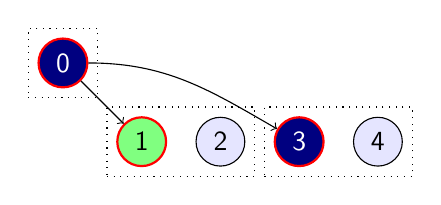
\begin{tikzpicture}
    \node[doc,active,fully](0) at (0,0){0};
    \node[doc,jshactive,fully](1) at (1,-1){1};
    \node[doc](2) at (2,-1){2};
    \node[doc,active,fully](3) at (3,-1){3};
    \node[doc](4) at (4,-1){4};
    \node[draw,dotted,fit=(0)] {};
    \node[draw,dotted,fit=(1)(2)] {};
    \node[draw,dotted,fit=(3)(4)] {};
    \draw[->](0)--(1);
    \draw[->](0)to[out=0,in=150](3);
  \end{tikzpicture}\]
  which traverses the history by $1$ to:
  \[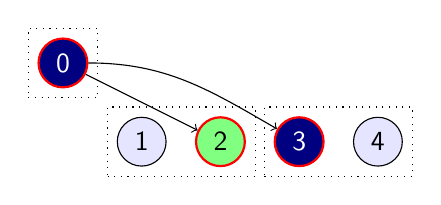
\begin{tikzpicture}
    \node[doc,active,fully](0) at (0,0){0};
    \node[doc](1) at (1,-1){1};
    \node[doc,jshactive,fully](2) at (2,-1){2};
    \node[doc,active,fully](3) at (3,-1){3};
    \node[doc](4) at (4,-1){4};
    \node[draw,dotted,fit=(0)] {};
    \node[draw,dotted,fit=(1)(2)] {};
    \node[draw,dotted,fit=(3)(4)] {};
    \draw[->](0)--(2);
    \draw[->](0)to[out=0,in=150](3);
  \end{tikzpicture}\]
  which traverses the history by $1$ to:
  \[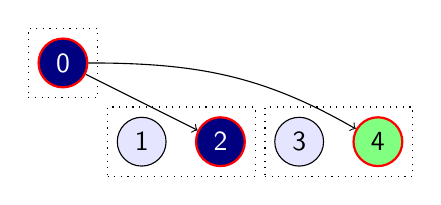
\begin{tikzpicture}
    \node[doc,active,fully](0) at (0,0){0};
    \node[doc](1) at (1,-1){1};
    \node[doc,active,fully](2) at (2,-1){2};
    \node[doc](3) at (3,-1){3};
    \node[doc,jshactive,fully](4) at (4,-1){4};
    \node[draw,dotted,fit=(0)] {};
    \node[draw,dotted,fit=(1)(2)] {};
    \node[draw,dotted,fit=(3)(4)] {};
    \draw[->](0)--(2);
    \draw[->](0)to[out=0,in=150](4);
  \end{tikzpicture}\]
  but $H$ traverses the history $2$ to:
  \[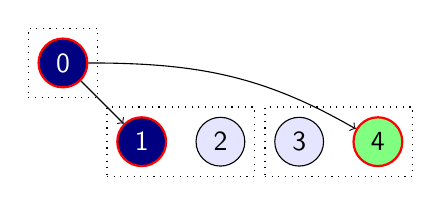
\begin{tikzpicture}
    \node[doc,active,fully](0) at (0,0){0};
    \node[doc,active,fully](1) at (1,-1){1};
    \node[doc](2) at (2,-1){2};
    \node[doc](3) at (3,-1){3};
    \node[doc,jshactive,fully](4) at (4,-1){4};
    \node[draw,dotted,fit=(0)] {};
    \node[draw,dotted,fit=(1)(2)] {};
    \node[draw,dotted,fit=(3)(4)] {};
    \draw[->](0)--(1);
    \draw[->](0)to[out=0,in=150](4);
  \end{tikzpicture}\]
\end{counterexample}
%
This counterexample is caused by the definition of `traverses the history by $\delta$' which
only traverses one document's session history. Instead, we should traverse
the history of all $\delta$ documents.

\begin{patch}
Define \emph{$\aNH$ traverses the history by $+\delta$ to $\aNH'$} when:
\begin{itemize}
\item the joint session future of $\aNH$ is $\aDoc_1 \ltChron \cdots \ltChron \aDoc_\delta \ltChron \cdots$,
\item there is some $\aNH=\aNH_0,\ldots,\aNH_\delta=\aNH'$, such that
\item $H_{i-1}$ traverses the history to $d_i$ in $H_i$ for each $1 \le i \le \delta$.
\end{itemize}
Define \emph{$\aNH$ traverses the history by $-\delta$ to $\aNH'$} when:
\begin{itemize}
\item the joint session past of $\aNH$ is $\aDoc_1 \gtChron \cdots \gtChron \aDoc_\delta \gtChron \cdots$,
\item there is some $\aNH=\aNH_0,\ldots,\aNH_\delta=\aNH'$, such that
\item $H_{i-1}$ traverses the history to $d_i$ in $H_i$ for each $1 \le i \le \delta$.
\end{itemize}
\end{patch}
Unfortunately, Goal~\ref{goal:homomorphism} is not satisfied,
even with this patch.
\begin{counterexample}
  Let $H$ be:
  \[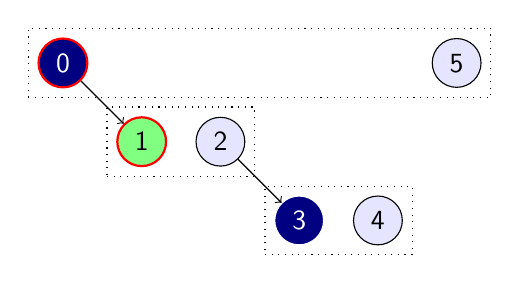
\begin{tikzpicture}
    \node[doc,active,fully](0) at (0,0){0};
    \node[doc,jshactive,fully](1) at (1,-1){1};
    \node[doc](2) at (2,-1){2};
    \node[doc,active](3) at (3,-2){3};
    \node[doc](4) at (4,-2){4};
    \node[doc](5) at (5,0){5};
    \node[draw,dotted,fit=(0)(5)] {};
    \node[draw,dotted,fit=(1)(2)] {};
    \node[draw,dotted,fit=(3)(4)] {};
    \draw[->](0)--(1);
    \draw[->](2)--(3);
  \end{tikzpicture}\]
  which moves forwards by $1$ to:
  \[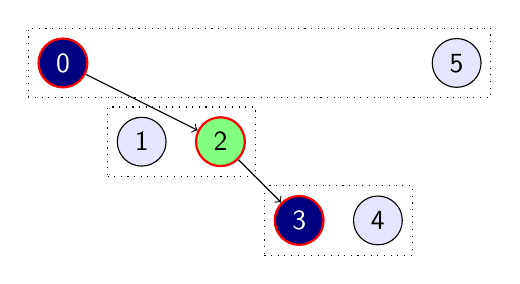
\begin{tikzpicture}
    \node[doc,active,fully](0) at (0,0){0};
    \node[doc](1) at (1,-1){1};
    \node[doc,jshactive,fully](2) at (2,-1){2};
    \node[doc,active,fully](3) at (3,-2){3};
    \node[doc](4) at (4,-2){4};
    \node[doc](5) at (5,0){5};
    \node[draw,dotted,fit=(0)(5)] {};
    \node[draw,dotted,fit=(1)(2)] {};
    \node[draw,dotted,fit=(3)(4)] {};
    \draw[->](0)--(2);
    \draw[->](2)--(3);
  \end{tikzpicture}\]
  which in turn moves forwards by $1$ to:
  \[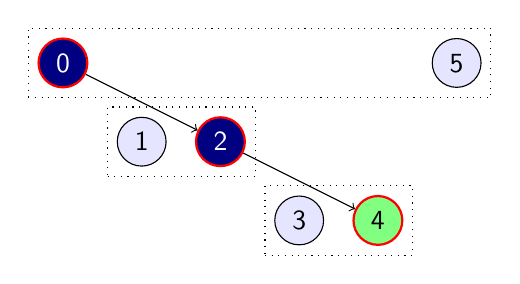
\begin{tikzpicture}
    \node[doc,active,fully](0) at (0,0){0};
    \node[doc](1) at (1,-1){1};
    \node[doc,active,fully](2) at (2,-1){2};
    \node[doc](3) at (3,-2){3};
    \node[doc,jshactive,fully](4) at (4,-2){4};
    \node[doc](5) at (5,0){5};
    \node[draw,dotted,fit=(0)(5)] {};
    \node[draw,dotted,fit=(1)(2)] {};
    \node[draw,dotted,fit=(3)(4)] {};
    \draw[->](0)--(2);
    \draw[->](2)--(4);
  \end{tikzpicture}\]
  but $H$ goes forward by $2$ to:
  \[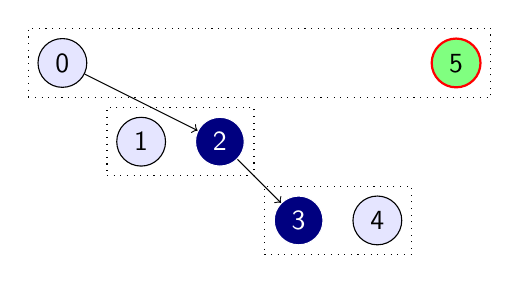
\begin{tikzpicture}
    \node[doc](0) at (0,0){0};
    \node[doc](1) at (1,-1){1};
    \node[doc,active](2) at (2,-1){2};
    \node[doc,active](3) at (3,-2){3};
    \node[doc](4) at (4,-2){4};
    \node[doc,jshactive,fully](5) at (5,0){5};
    \node[draw,dotted,fit=(0)(5)] {};
    \node[draw,dotted,fit=(1)(2)] {};
    \node[draw,dotted,fit=(3)(4)] {};
    \draw[->](0)--(2);
    \draw[->](2)--(3);
  \end{tikzpicture}\]
\end{counterexample}
The problem this time is that the definition of `joint session history' only includes
the fully active documents, not all active documents.

\begin{patch}
Define:
\begin{itemize}
\item the \emph{joint session future} is $\{ \bDoc \mid \exists \aDoc \in \Active \st \aDoc \ltSess \bDoc \}$, and
\item the \emph{joint session past} is $\{ \bDoc \mid \exists \aDoc \in \Active \st \aDoc \gtSess \bDoc \}$.
\end{itemize}
\end{patch}

\begin{goal}
  If $\aDoc$ in $\aNH$ navigates to $\aDoc'$ in $\aNH'$,
  and $\aNH'$ traverses the history by $-1$ to $\aNH''$,
  then $\FullyActive=\FullyActive''$.
\end{goal}

\begin{counterexample}
  \[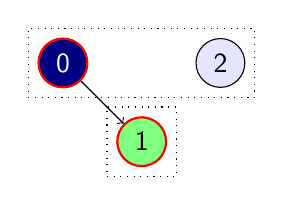
\begin{tikzpicture}
    \node[doc,active,fully](0) at (0,0){0};
    \node[doc,jshactive,fully](1) at (1,-1){1};
    \node[doc](2) at (2,0){2};
    \node[draw,dotted,fit=(0)(2)] {};
    \node[draw,dotted,fit=(1)]{};
    \draw[->](0)--(1);
  \end{tikzpicture}\]
  navigates 1 to 3 in:
  \[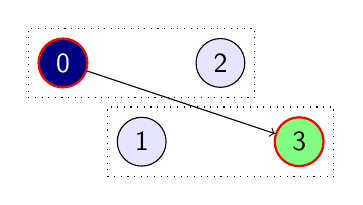
\begin{tikzpicture}
    \node[doc,active,fully](0) at (0,0){0};
    \node[doc](1) at (1,-1){1};
    \node[doc](2) at (2,0){2};
    \node[doc,jshactive,fully](3) at (3,-1){3};
    \node[draw,dotted,fit=(0)(2)] {};
    \node[draw,dotted,fit=(1)(3)]{};
    \draw[->](0)--(3);
  \end{tikzpicture}\]
  which traverses the history by $-1$ to:
  \[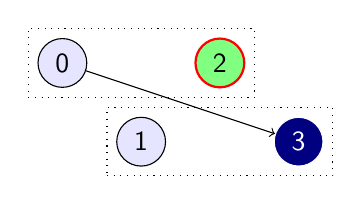
\begin{tikzpicture}
    \node[doc](0) at (0,0){0};
    \node[doc](1) at (1,-1){1};
    \node[doc,jshactive,fully](2) at (2,0){2};
    \node[doc,active](3) at (3,-1){3};
    \node[draw,dotted,fit=(0)(2)] {};
    \node[draw,dotted,fit=(1)(3)]{};
    \draw[->](0)--(3);
  \end{tikzpicture}\]
\end{counterexample}

\begin{counterexample}
  \[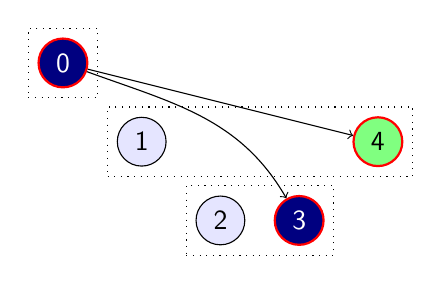
\begin{tikzpicture}
    \node[doc,active,fully](0) at (0,0){0};
    \node[doc](1) at (1,-1){1};
    \node[doc](2) at (2,-2){2};
    \node[doc,active,fully](3) at (3,-2){3};
    \node[doc,jshactive,fully](4) at (4,-1){4};
    \node[draw,dotted,fit=(0)]{};
    \node[draw,dotted,fit=(1)(4)]{};
    \node[draw,dotted,fit=(2)(3)]{};
    \draw[->](0)--(4);
    \draw[->](0)to[out=-20,in=120](3);
  \end{tikzpicture}\]
  which traverses the history by $-1$ to:
  \[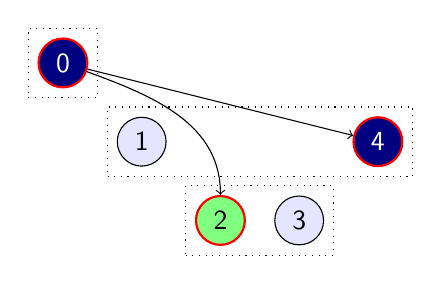
\begin{tikzpicture}
    \node[doc,active,fully](0) at (0,0){0};
    \node[doc](1) at (1,-1){1};
    \node[doc,jshactive,fully](2) at (2,-2){2};
    \node[doc](3) at (3,-2){3};
    \node[doc,active,fully](4) at (4,-1){4};
    \node[draw,dotted,fit=(0)]{};
    \node[draw,dotted,fit=(1)(4)]{};
    \node[draw,dotted,fit=(2)(3)]{};
    \draw[->](0)--(4);
    \draw[->](0)to[out=-20,in=90](2);
  \end{tikzpicture}\]
  which traverses the history by $-1$ to:
  \[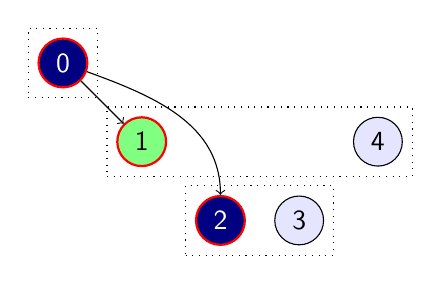
\begin{tikzpicture}
    \node[doc,active,fully](0) at (0,0){0};
    \node[doc,jshactive,fully](1) at (1,-1){1};
    \node[doc,active,fully](2) at (2,-2){2};
    \node[doc](3) at (3,-2){3};
    \node[doc](4) at (4,-1){4};
    \node[draw,dotted,fit=(0)]{};
    \node[draw,dotted,fit=(1)(4)]{};
    \node[draw,dotted,fit=(2)(3)]{};
    \draw[->](0)--(1);
    \draw[->](0)to[out=-20,in=90](2);
  \end{tikzpicture}\]
  which traverses the history by $1$ to:
  \[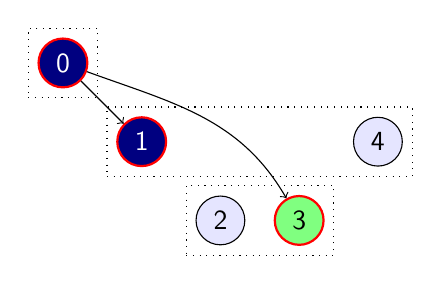
\begin{tikzpicture}
    \node[doc,active,fully](0) at (0,0){0};
    \node[doc,active,fully](1) at (1,-1){1};
    \node[doc](2) at (2,-2){2};
    \node[doc,jshactive,fully](3) at (3,-2){3};
    \node[doc](4) at (4,-1){4};
    \node[draw,dotted,fit=(0)]{};
    \node[draw,dotted,fit=(1)(4)]{};
    \node[draw,dotted,fit=(2)(3)]{};
    \draw[->](0)--(1);
    \draw[->](0)to[out=-20,in=120](3);
  \end{tikzpicture}\]
  which traverses the history by $1$ to:
  \[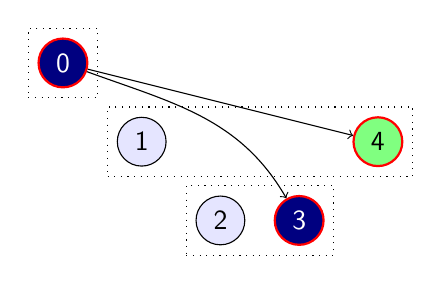
\begin{tikzpicture}
    \node[doc,active,fully](0) at (0,0){0};
    \node[doc](1) at (1,-1){1};
    \node[doc](2) at (2,-2){2};
    \node[doc,active,fully](3) at (3,-2){3};
    \node[doc,jshactive,fully](4) at (4,-1){4};
    \node[draw,dotted,fit=(0)]{};
    \node[draw,dotted,fit=(1)(4)]{};
    \node[draw,dotted,fit=(2)(3)]{};
    \draw[->](0)--(4);
    \draw[->](0)to[out=-20,in=120](3);
  \end{tikzpicture}\]
\end{counterexample}

\section{Experiments}

[A write-up of CGB's experiments with how different browsers handle navigation.]

\section{Specification}

[Suggested edits to the spec:
  1. traverse to each document, not just the selected one,
  2. keep all documents in the seession history, not just the fully active ones,
  3. change the session history order.]

\section{Conclusion}

[We did stuff.]

\end{document}
